\section{Models}

This section will introduce the proposed models for the two sub-tasks of symptom identification: \textit{relevance judgment} and \textit{status inference} that can leverage the data from multiple diseases simultaneously, and how to leverage the above models for \textit{mental disease detection}.

\subsection{Symptom Relevance Judgment}
\label{sec:model_rel}
The task of relevance judgment can be viewed as a multi-label classification problem, where we need to predict for each symptom if it is relevant to the sentence. However, when we want to train the model on the annotations from different diseases, we will face the problem of \textit{missing labels}, as we will not annotate the relevance of symptom $s$ in the dataset of disease $d$ if $s$ is not considered to be a typical symptom of $d$. A naive solution is to treat all such missing labels as negative. However, since the 
co-existence of multiple diseases on the same person is not uncommon, it is likely that the 
typical symptom of other diseases will also be present. Therefore, 
such solution will lead to false negatives and harm the model performance. 

Inspired by \citet{fonseca2020addressing} and \citet{gururani2021semi}, we experimented with two techniques to address the problem of missing labels.

\paragraph{Loss Masking} Missing labels will be ignored during the loss calculation. This can prevent the model from learning incorrect negative labels, but also restricted the exploitation of the true negatives among missing labels.

\paragraph{Label Enhancement} This method involves two-stage trainings of a teacher model and a student model. First, a teacher model is trained using \textit{Loss Masking}. Then we use the teacher model to predict the probabilities of the missing labels in the training set. If the predicted probability of a symptom is lower than certain threshold, we change its label to negative, otherwise it will still be treated as missing. A second student model will be trained on the enhanced labels together with \textit{Loss Masking}. In contrast to previous works which set the threshold to enhance the missing labels with top $k\%$ confidence, we search for the cutting point where the teacher model can achieve 90\% True Negative Rate on the ROC curve of existing annotations as the threshold for each symptom, which can quantitatively guarantee the quality of the enhanced labels.

Overall, we use a BERT-based encoder \citep{devlin2018bert} with a linear layer on top of the representation of \texttt{[CLS]} to predict the probabilities of all symptoms
with a sigmoid activation, and train the model with binary cross entropy loss against the labels adjusted with the methods above.

When trained on PsySym with control posts, the especially unbalanced positive/negative ratio can make the training hard. We thus additionally implement a \textit{Balanced Sampler} which samples equal amount of annotated sentences and control sentences for each batch.

\subsection{Symptom Status Inference}
\label{sec:model_status}
Status Inference aims to predict if the symptoms relevant to the sentence are truly present instead of being a negation (e.g. denying or recovery) or an uncertain guess. Therefore, it is natural to formulate it as a single-label binary classification problem. However, due to the ambiguity in the expression,
% on social media (as opposed to the precise terms used in medical records)
lack of context and the different understandings of annotators, the agreement on the status labels are relatively low (\S \ref{sec:data_annotation}) despite our quality control efforts. Consequently, even if we can derive binary labels from the majority voting of annotators, models trained on such ambiguous targets will hardly show satisfying performance. % \footnote{In our preliminary experiments, the F1 score of the experimented models are close to 0.}

However, we may not simply attribute such disagreement to poor annotation quality, since there is inherent ambiguity in the annotations of natural language inference tasks, as is reported by \citet{nie2020can}. We can still make reasonable probabilistic estimation of the status by embracing the ambiguity and directly learn from the annotation distribution \citep{meissner2021embracing}. Therefore, we change the learning target from binary labels to the portion of annotators who label the status as \textit{uncertain}, and the possible values are thus 0, 1/3, 2/3 and 1. Then we use BERT-based model with sigmoid activation and cross entropy loss to predict the non-binary labels. 

\subsection{Mental Disease Detection}
\label{sec:disease_detect}

\begin{figure}[h]
    \centering
    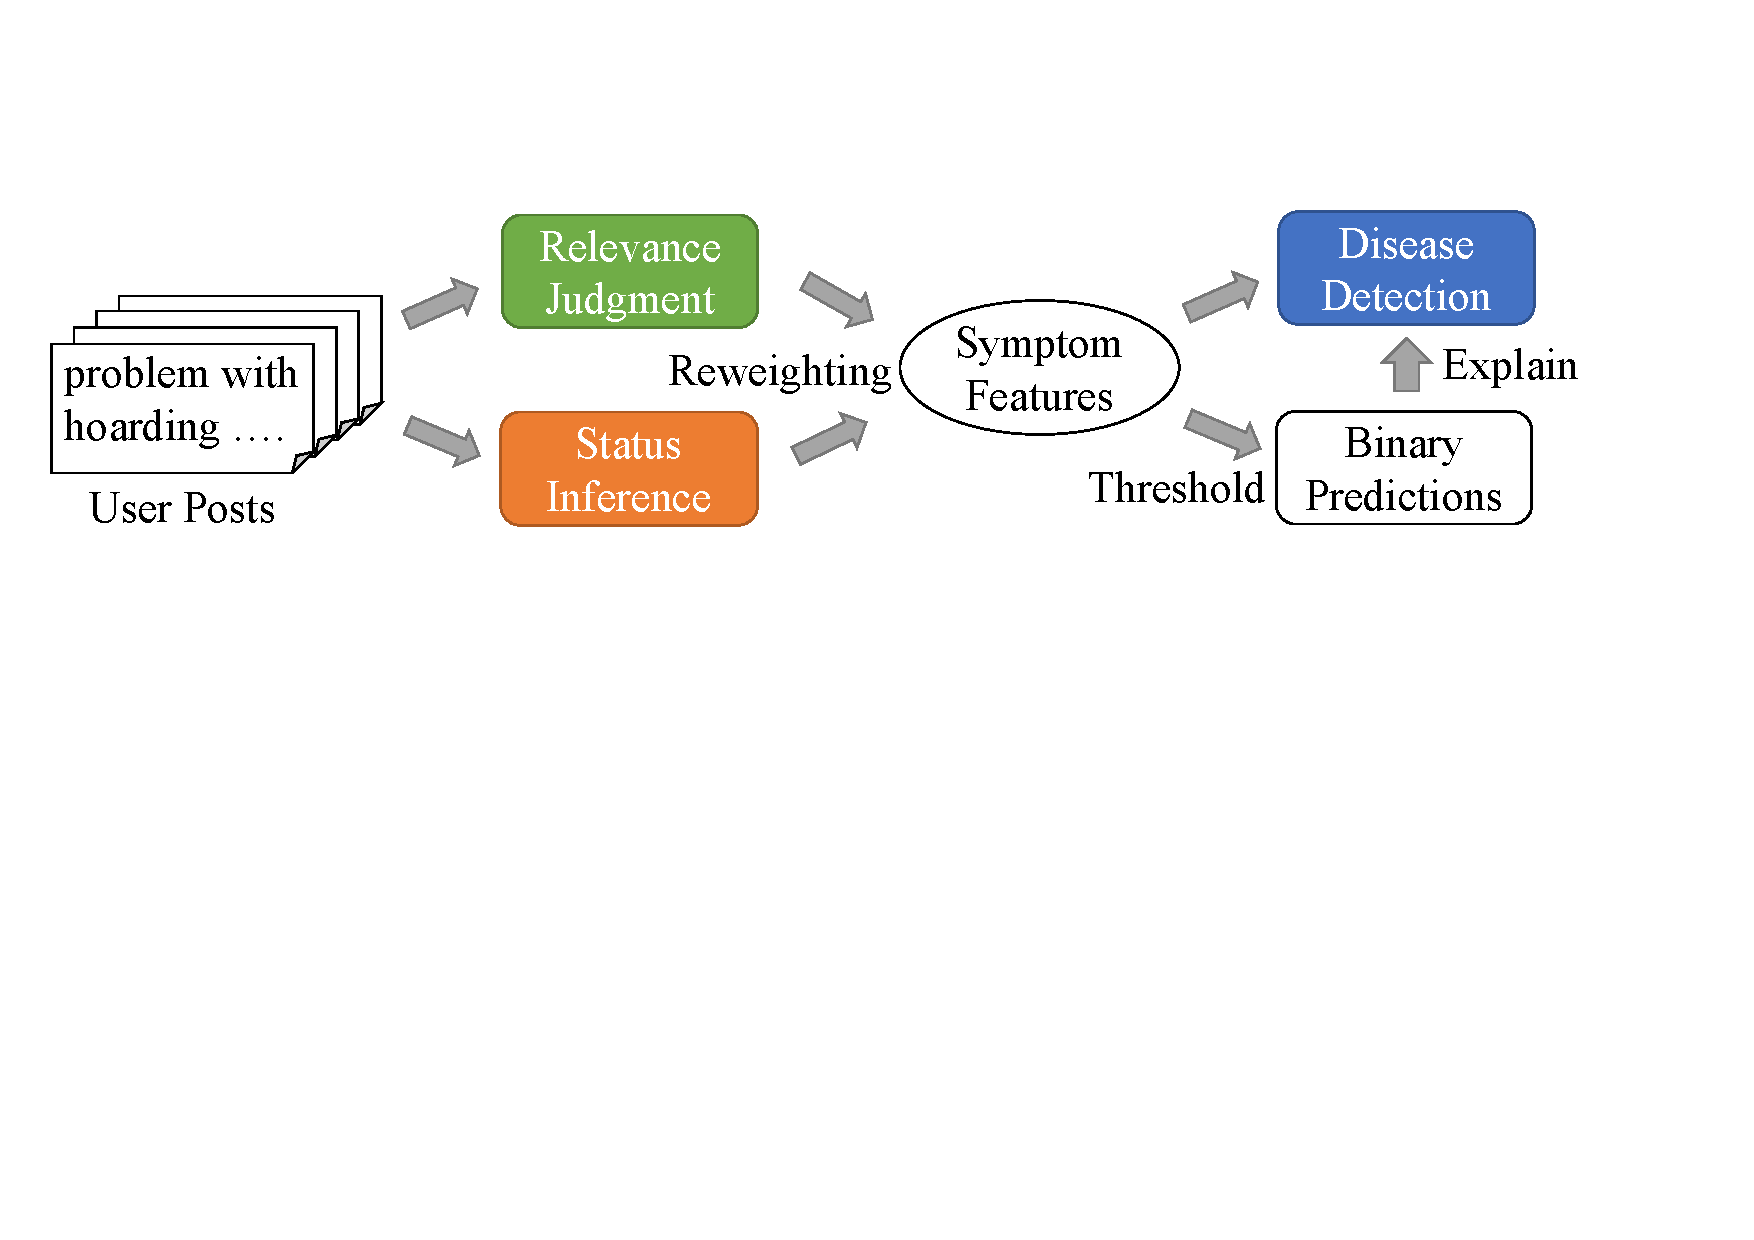
\includegraphics[width=1.0\columnwidth]{figures/mdd_pipeline.pdf}
    \caption{The proposed symptom-assisted MDD pipeline.}
    \label{fig:mdd_pipeline}
\end{figure}

The task of MDD is to predict if a user suffers from certain mental diseases with his/her posting history. Figure \ref{fig:mdd_pipeline} illustrates the proposed symptom-assisted MDD pipeline. First, we utilize the predicted probabilities from relevance judgment models trained on PsySym as the extracted symptom features. 

Next, to further improve the symptom features, we also introduce \textit{subject} and \textit{status} feature. The \textit{subject} feature is a binary variable indicating if the discussed symptoms of a post is about the poster himself. We calculate this feature by counting the mentions/pronouns of other people and the use of first person pronouns, and set the feature as 1 if the latter is no less than the former. The \textit{status} feature is the predicted probability of the status inference model that the symptoms are present. It is obvious that a post not about the poster himself or exhibiting symptoms clearly should not count much to disease detection. We thus experiment with the \textbf{Reweighting} approach similar to \citet{karmen2015screening} to incorporate them into the symptom features:
\begin{equation}
    f_{symp} = p_{rel} \times w_{status} \times w_{subj}
\end{equation}
where $p_{rel}$ is the probabilities predicted by the relevance model; $w_{status}$ is the probability predicted by the status model; $w_{subj} = 0.9$ if the subject is the poster, otherwise $w_{subj} = 0.1$.

To conduct MDD, we incorporate these features into the model proposed by \citet{nguyen2022improving}. This model utilizes CNN of various kernel sizes on top of the sequence of feature vectors extracted from a user's posting list to aggregate the information from consecutive posts. The features can either be pure-text features like the sentence embeddings from pretrained BERT, or the proposed symptom features (denoted as \textbf{Symp} below). Note that the symptom features can be much more condense than pure-text features (38-dim symptom probabilities versus 768-dim BERT embedding).

Finally, for the ease of explaining MDD results with symptoms (\S \ref{sec:interpret}), we may need binary decision on the their presence. To achieve this, we use 0.5 to threshold on the reweighted symptom features, where the re-weighting procedure can help eliminate posts that should not be counted for the diagnose. 
